% !Mode:: "TeX:UTF-8"
% !TEX program  = xelatex
\section{Introduction}

\subsection{single cell RNA sequencing}

In the past decades, bulk cell RNA sequencing was extensively used to study the gene expression features at the tissue level. However, it only reflects the averaged expression level of cells in a tissue. The rapid growth of single-cell RNA sequencing (scRNA-seq) technologies enables researchers to study the gene expression patterns at the single-cell level. It dramatically aids researchers in identifying molecular heterogeneity and better understand biological mechanisms \cite{shapiro2013single}. For example, the single-cell sequencing of cancer cells reveals the mutations on each sub-population of cells and helps construct the cancer development trajectory. 

\begin{figure}[htb!]
    \centering
    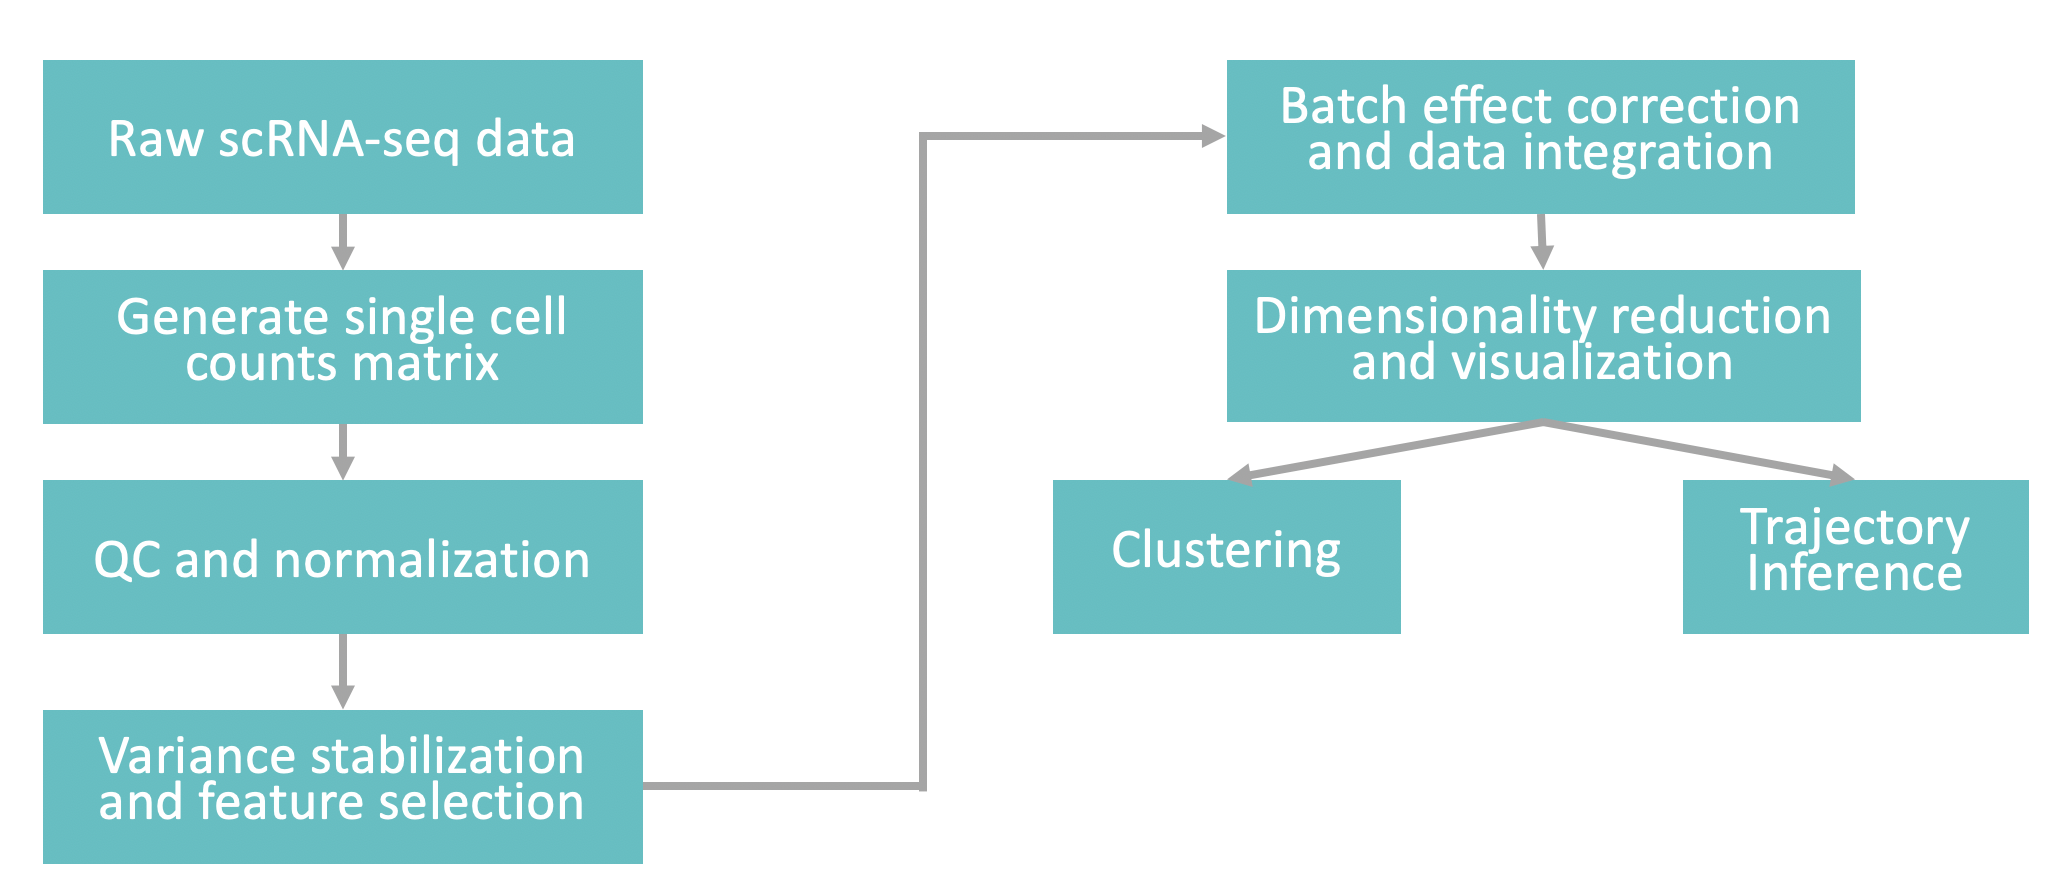
\includegraphics[width=1\textwidth]{figures/myfigures/scpip.png}
    \caption{The basic pipeline of scRNA-seq data analysis}
    \label{scpip}
\end{figure}

The primary pipeline of scRNA-seq analysis is shown in figure \ref{scpip}. Firstly, the raw sequencing FASTQ files should be processed to a count matrix. In this process, each read's sequence is aligned to a reference genome to find out the gene that read belongs to. Then, identify the corresponding cell by the cell barcode in the sequence. In this way, the count matrix can be generated \cite{petukhov2017accurate}. The value at the $i^{th}$ row and $j^{th}$ column is the expression value of gene $j$ at the cell $i$.

After getting a count matrix, quality control should be performed to remove technical biases and noises \cite{van2017single}. It usually involves removing dead cells by filtering out the cells with low reads or high mitochondrial reads and removing doublets. Also, a proper normalization, such as total count normalization or Sctransform normalization, helps identify additional cell heterogeneity \cite{vallejos2017normalizing}. Besides from normalization, variance stabilization and batch effect removing also make the downstream analysis easier.

The downstream analysis mainly consists of dimensionality reduction, clustering, trajectory inference, and cell-type annotation. Dimensionality reduction can represent the high dimensional scRNA-seq data in a low-dimensional space and thus benefit clustering and trajectory inference processes. scRNA-seq datasets usually contain some distinct cell types or the cells in continuous changes. For the cells that can be divided into several discrete types, cluster clustering can be performed to assign each cell to a cluster with the same type of cells. The most common clustering method for single-cell sequencing data is the Louvain algorithm \cite{traag2019louvain}. It uses a community detection algorithm to add data points to communities iteratively and thus clusters the cells. For those continuous cell types, trajectory inference is usually performed to resolve the cell development lineage. Monocle2 uses reverse graph embedding to learn the graph structure of the data in a high dimensional space and a low dimensional space at the same time \cite{qiu2017reversed}. Clustering and trajectory inference is usually performed based on the result of dimensionality reduction. Finally, cell type annotation is usually performed by identifying the genes that are uniquely expressing in a cluster and match the gene to the database of empirical cell type markers \cite{abdelaal2019comparison}. 

\subsection{Dimensionality reduction}

The single-cell sequencing data usually have more than two thousand dimensions, which makes it challenging to be analyzed directly. Thus, finding a meaningful low dimensional representation to represent those cell states is a necessary step in scRNA-seq data analyzing. Those genes are highly regulated and co-expressed. There is much redundant information in the dataset because only a limited number of cell states are in a group of cells. It is assumed that those data form a low dimensional manifold in a high dimensional space. The dimensionality reduction process can extract the crucial information in the original high dimensional data and represent it as a low-dimensional structure \ref{dr1}.  It plays a vital role in data visualization and data preprocessing, which allows efficient downstream analysis such as trajectory inference \cite{Saelens2019}, cell clustering \cite{weber2016comparison}, and cell sub-population identification \cite{Hwang2018}. 

\begin{figure}[htb!]
    \centering
    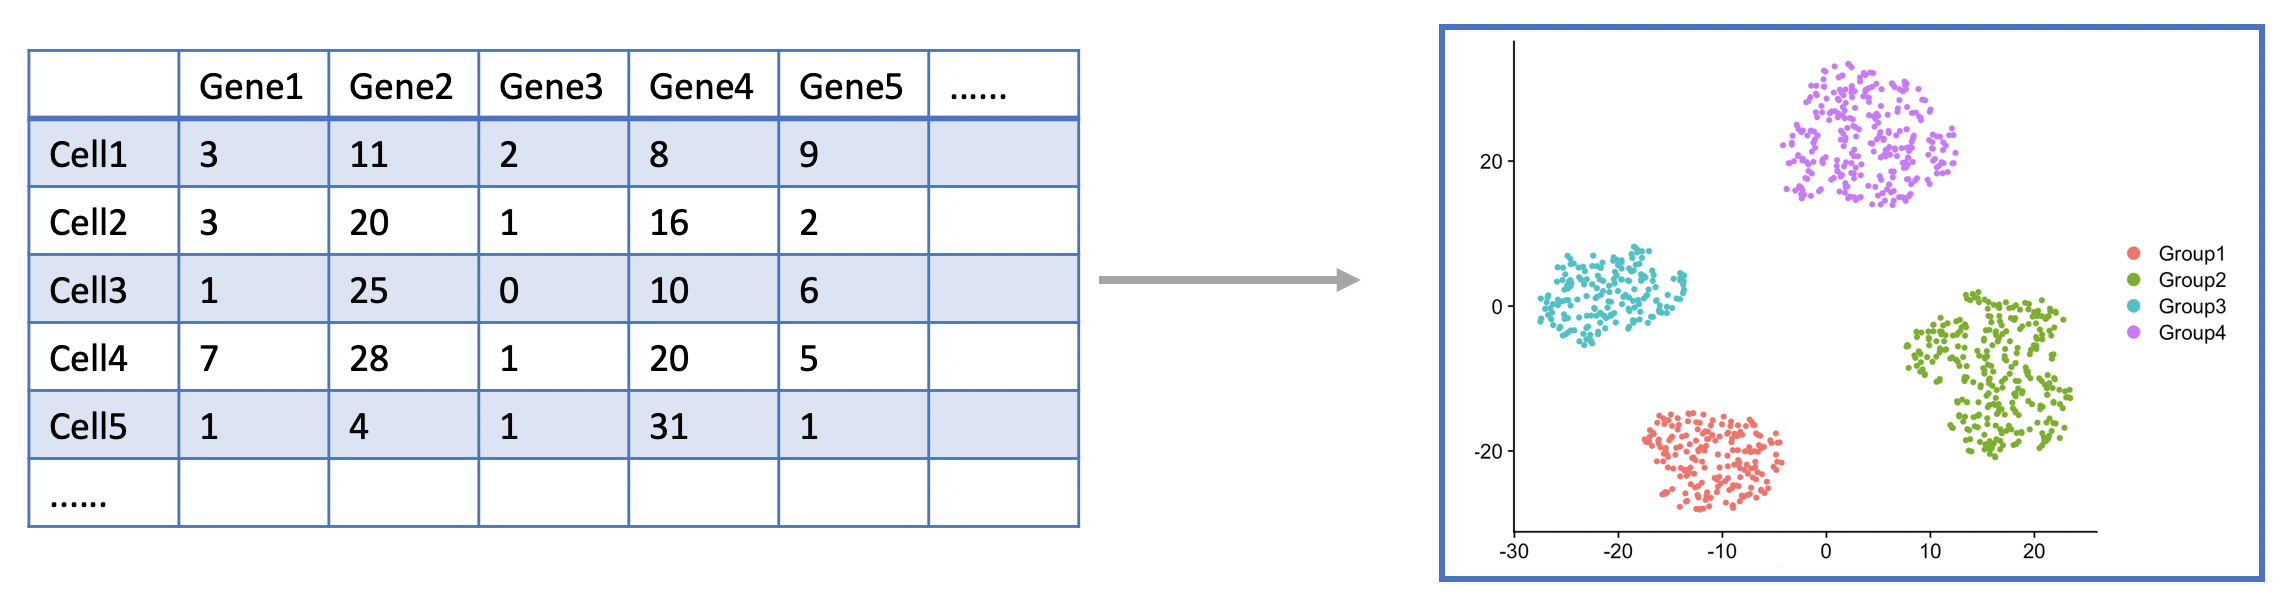
\includegraphics[width=1\textwidth]{figures/myfigures/dr1.png}
    \caption{Dimensionality reduction of sequencing data}
    \label{dr1}
\end{figure}

For example, Seurat uses PCA \cite{Abdi2010} to reduce dimensionality before clustering \cite{Satija2015}. Destiny \cite{angerer2016destiny} uses diffusion map before clustering. Monocle \cite{Qiu2017} performs uniform manifold approximation and projection (UMAP) \cite{McInnes2018} or independent component analysis (ICA) \cite{hyvarinen2000independent} before inferencing cell trajectories. 

The most classic and most common dimensionality reduction method is principal component analysis (PCA). PCA performs dimensionality reduction by iteratively finding the direction that can explain most variance and project points to that direction as a component. The first two principal components are usually chosen as coordinates to visualize data points. However, scRNA-seq datasets are usually non-linear because the relationship between genes is often non-linear. Thus, the linear dimensionality reduction methods such as PCA and MDS \cite{Kruskal1964} have some limitations. Non-linear methods usually have better performance for visualization of scRNA-seq data.

The most popular non-linear dimensionality reduction method is t-distributed stochastic neighbor embedding (tSNE). It calculates the similarity between data points in high dimensional space and low dimensional space and tries to keep the similarity distribution in two spaces as close as possible. By recovering the similarity relationships between cells, tSNE can considerably preserve local structures and can form delicate clusters in visualization.  However, tSNE cannot preserve global structures well. The size and spatial relationship of clusters are often random \cite{wattenberg2016how}. Another non-linear dimensionality reduction method UMAP is developed in recent years. It has a similar visualization performance with tSNE \cite{kobak2019umap} but have lower running time and more reproducibility than tSNE \cite{becht2019dimensionality}.

\subsection{Dropout events}

However, the single-cell sequencing data have more noise than bulk cell data because of the low RNA capture efficiency and incomplete reverse transcription in single-cell sequencing \cite{Peng2019}. Some studies estimate that only 10\%-15\% of RNA in a cell can be captured and transcribed \cite{zheng2017massively}. Thus, single-cell sequencing data usually have excessive dropouts, which means many data points that should have more significant value are presented as zero or a value lower than the exact expression, which is shown in figure \ref{dropout}.

\begin{figure}[htb!]
    \centering
    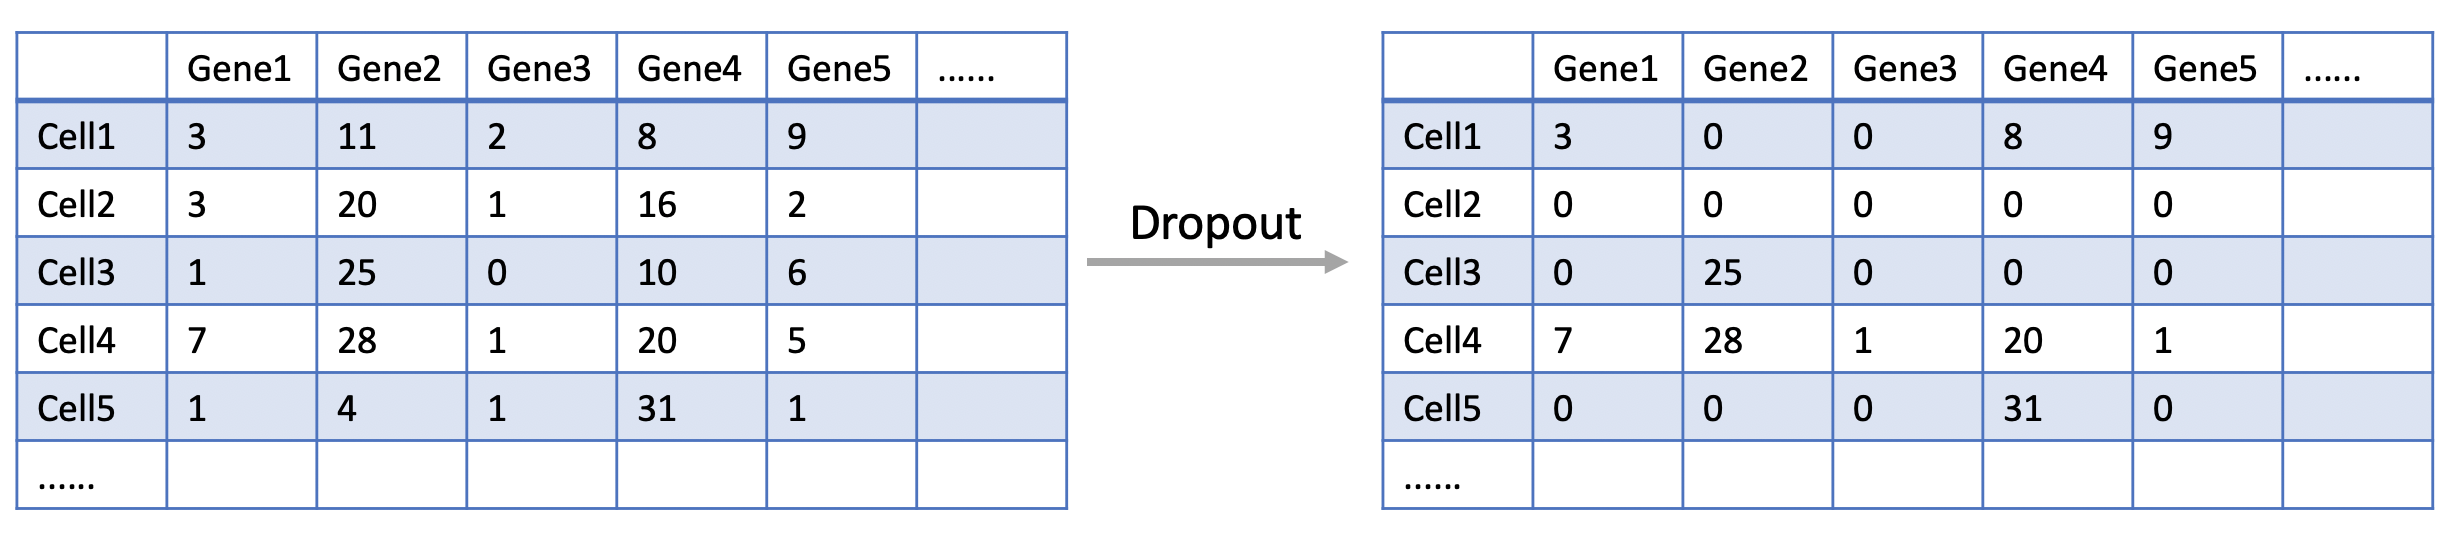
\includegraphics[width=1\textwidth]{figures/myfigures/dropout.png}
    \caption{The process of dropout to scRNA-seq data}
    \label{dropout}
\end{figure}

Some traditional methods cannot effectively extract the features which cause dimensionality reduction more difficult because of these noises. The visualization performance also decreases. Sometimes, the data points get mixed, sometimes it can be separated but is very dispersed, such as in figure \ref{dr2}.

\begin{figure}[htb!]
    \centering
    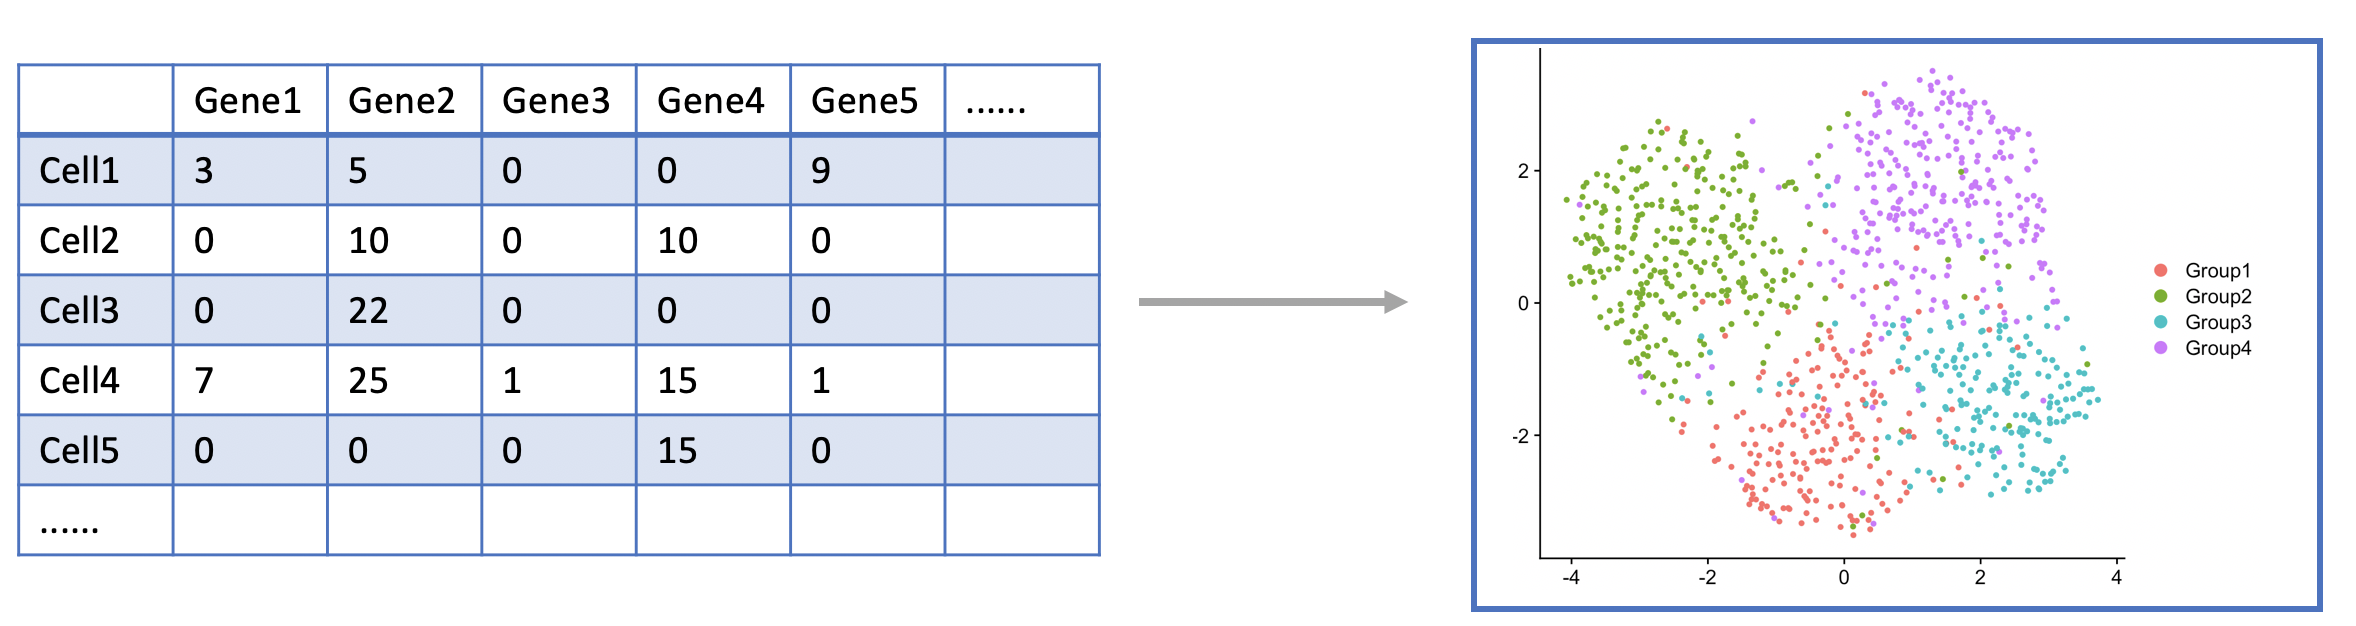
\includegraphics[width=1\textwidth]{figures/myfigures/dr2.png}
    \caption{Dimensionality reduction of scRNA-seq data with dropouts}
    \label{dr2}
\end{figure}

Many imputation methods are developed recently to impute those missing points. One kind of strategy, including MAGIC \cite{van2017magic}, RESCUE \cite{Tracy2019}, scImpute \cite{Li2018} and DrImpute \cite{gong2018drimpute}, borrows information of the same gene from other similar cells that don't have dropouts on that gene. Similar cells are chosen based on the genes that are unlikely to be affected by dropouts.

Some strategy performs imputation and clustering or dimensionality reduction at the same time \cite{lin2017cidr}. For example, ZIFA \cite{Pierson2015} performs dimensionality reduction while imputing the missing values at the same time. It probabilistically models the conditional dropout events and uses the EM algorithm \cite{mclachlan2007algorithm} to refer the model parameters and latent variables iteratively. 

With the fast development of deep learning in recent years, some approaches make use of deep learning technologies. scScope \cite{Deng2019} uses a recurrent neuron network to impute the missing values. scGAIN \cite{gunady2019scgain} uses a generative adversarial network (GAN) to learn the distribution of the scRNA-seq data and impute the missing values. GraphSCI \cite{rao2020imputing} uses graph convolution neuron network and makes use of gene-gene interaction to impute scRNA-seq data. Moreover, some methods build the model based on autoencoder or variational autoencoder. In this way, the bottleneck layer can be used for dimensionality reduction. For example, VASC \cite{Wang2018} adds the dropout model in ZIFA to a VAE model to enable it to model the dropout events. DCA \cite{Eraslan2019a} uses autoencoder to impute the missing values by assuming the zero-inflated negative binomial model \cite{Hafemeister2019}. 

\subsection{ZIVA model}
In this study, I compared the performance of several popular dimensionality reduction methods on visualization, clustering, and trajectory inference of scRNA-seq data. Also, based on the structure of VAE \cite{Kingma2014}, I improved the model of VASC \cite{Wang2018} and proposed a new method, zero-inflated variational autoencoder (ZIVA), to analyze and visualize the single-cell RNA sequencing data. It uses the Gumbel softmax and double-exponential function to model the dropout events. The comparison results show that ZIVA has excellent performance on cell clustering and cell trajectory inference tasks.